% Gabarit pandoc des corrigés publiés (brut et guidé). Contenu sans marque ni nom de site.
% Compilation : lualatex (latexmk -lualatex).
% Le Markdown reste la source unique : ne pas éditer ce fichier .tex à la main.
\documentclass[11pt,a4paper]{article}

% --- Moteur, polices (Latin Modern) et langue ---------------------------------
\usepackage{iftex}
\ifLuaTeX\else\errmessage{Ce document se compile avec lualatex}\fi
\usepackage{amsmath,amssymb,mathtools}
\usepackage{fontspec}
% mathrm=sym : \mathrm prend ses glyphes dans la police mathématique (ℓ, μ, Ω), comme KaTeX.
\usepackage[math-style=TeX,bold-style=TeX,mathrm=sym]{unicode-math}
% Repli pour les glyphes absents de Latin Modern (indices et exposants Unicode,
% flèches, filets des schémas en texte, symboles) : DejaVu, puis Latin Modern Math
% (ℓ, lettres mathématiques Unicode des légendes).
\directlua{
  luaotfload.add_fallback("repliTexte", {"DejaVuSerif:mode=harf;", "DejaVuSans:mode=harf;", "file:latinmodern-math.otf:mode=harf;"})
  luaotfload.add_fallback("repliMono", {"DejaVuSansMono:mode=harf;", "DejaVuSans:mode=harf;", "file:latinmodern-math.otf:mode=harf;"})
}
\setmainfont{Latin Modern Roman}[RawFeature={fallback=repliTexte}]
\setsansfont{Latin Modern Sans}[RawFeature={fallback=repliTexte}]
\setmonofont{Latin Modern Mono}[RawFeature={fallback=repliMono}]
\setmathfont{Latin Modern Math}
\usepackage[french]{babel}
\frenchsetup{SmallCapsFigTabCaptions=false}

% --- Mise en page --------------------------------------------------------------
\usepackage[a4paper,margin=2.2cm,headheight=14pt,footskip=1.2cm]{geometry}
\usepackage{microtype}
\setlength{\emergencystretch}{4em}
\tolerance=1500
\setlength{\parindent}{0pt}
\setlength{\parskip}{0.55\baselineskip plus 2pt minus 1pt}
\usepackage{xcolor}
% Gris nommés : babel-french rend « ! » actif dans le document.
\definecolor{gris2}{gray}{0.98}
\definecolor{gris3}{gray}{0.97}
\definecolor{gris5}{gray}{0.95}
\definecolor{gris35}{gray}{0.65}
\definecolor{gris40}{gray}{0.60}
\definecolor{gris45}{gray}{0.55}
\definecolor{gris50}{gray}{0.50}
\definecolor{gris55}{gray}{0.45}
\definecolor{gris60}{gray}{0.40}
\definecolor{gris65}{gray}{0.35}
\definecolor{gris70}{gray}{0.30}
\definecolor{gris80}{gray}{0.20}
\definecolor{gris85}{gray}{0.15}
\usepackage{graphicx}
\usepackage{float}
\usepackage{caption}
\captionsetup{font=small,labelformat=empty,justification=centering}
\usepackage{booktabs,longtable,array,multirow,calc}
\usepackage{siunitx}
\sisetup{locale=FR}
\usepackage[version=4]{mhchem}
\usepackage{listings}
\usepackage{fancyhdr}
\usepackage{lastpage}
\usepackage[most]{tcolorbox}
\usepackage{enumitem}
\setlist{nosep,leftmargin=*,topsep=2pt}
\usepackage[hidelinks,unicode]{hyperref}
\usepackage{bookmark}
\hypersetup{pdftitle={X-ENS MPI — Physique MPI 2026},pdfauthor={Rédigé par IA},pdfcreator={LaTeX},pdfsubject={Corrigé brut}}
\usepackage{xurl}

% --- Pandoc : listes, tableaux, figures ----------------------------------------
\providecommand{\passthrough}[1]{#1}
\providecommand{\tightlist}{\setlength{\itemsep}{0pt}\setlength{\parskip}{0pt}}

\makeatletter
\def\maxwidth{\ifdim\Gin@nat@width>\linewidth\linewidth\else\Gin@nat@width\fi}
\def\maxheight{\ifdim\Gin@nat@height>0.55\textheight 0.55\textheight\else\Gin@nat@height\fi}
\makeatother
\setkeys{Gin}{width=\maxwidth,height=\maxheight,keepaspectratio}
\setcounter{secnumdepth}{-\maxdimen}
\providecommand{\pandocbounded}[1]{#1}
\usepackage{longtable,booktabs,array}

% --- Code (listings) -----------------------------------------------------------
\lstset{
  basicstyle=\ttfamily\small,
  columns=fullflexible,
  keepspaces=true,
  breaklines=true,
  breakatwhitespace=false,
  postbreak=\mbox{\textcolor{gris50}{$\hookrightarrow$}\space},
  frame=single,
  rulecolor=\color{gris35},
  framesep=4pt,
  xleftmargin=5pt,xrightmargin=5pt,
  backgroundcolor=\color{gris3},
  keywordstyle=\bfseries,
  commentstyle=\color{gris65},
  stringstyle=\color{gris80},
  showstringspaces=false,
  tabsize=4,
  extendedchars=true,
  aboveskip=6pt,belowskip=6pt,
}

% --- Macros des corrigés (KaTeX ↔ LaTeX) ---------------------------------------
% Les corrigés sont écrits pour KaTeX : on définit ici ce que KaTeX connaît et
% que LaTeX n'a pas, sans jamais retoucher le Markdown.
\providecommand{\R}{\mathbb{R}}
\providecommand{\N}{\mathbb{N}}
\providecommand{\Z}{\mathbb{Z}}
\providecommand{\Q}{\mathbb{Q}}
\providecommand{\C}{\mathbb{C}}
\providecommand{\dd}{\mathrm{d}}
\providecommand{\llbracket}{\lBrack}
\providecommand{\rrbracket}{\rBrack}
\providecommand{\lBrace}{\lbrace}
\providecommand{\rBrace}{\rbrace}
\providecommand{\Box}{\square}
\providecommand{\Diamond}{\lozenge}
\providecommand{\varnothing}{\emptyset}
\providecommand{\argmax}{\operatorname*{arg\,max}}
\providecommand{\argmin}{\operatorname*{arg\,min}}
\renewcommand{\leq}{\leqslant}
\renewcommand{\geq}{\geqslant}

% Équation hors texte : réduite à la largeur de la ligne si elle déborde.
\newsavebox{\boiteequation}
\newcommand{\equationajustee}[1]{%
  \sbox{\boiteequation}{$\displaystyle #1$}%
  \ifdim\wd\boiteequation>\linewidth
    \[\resizebox{\linewidth}{!}{\usebox{\boiteequation}}\]%
  \else
    \[#1\]%
  \fi}

% --- Encadrés pédagogiques (sobres, lisibles en noir et blanc) -----------------
\tcbset{
  encadre/.style={
    enhanced,breakable,sharp corners,
    colback=white,colframe=gris55,
    boxrule=0.4pt,leftrule=2.2pt,
    left=6pt,right=6pt,top=3pt,bottom=3pt,
    before skip=6pt,after skip=6pt,
    fonttitle=\bfseries\small,coltitle=black,
    attach title to upper,after title={\quad},
    parbox=false,
  }
}
\newtcolorbox{indication}[1]{encadre,colframe=gris45,colback=gris2,title={Indication~#1}}
\newtcolorbox{methode}{encadre,colframe=gris70,title={Méthode}}
\newtcolorbox{piege}{encadre,colframe=gris85,boxrule=0.8pt,leftrule=2.2pt,title={Piège}}
\newtcolorbox{jury}{encadre,colframe=gris60,colback=gris5,title={Jury}}
\newtcolorbox{encadrenote}{encadre,colframe=gris40}

% --- Titres de section ---------------------------------------------------------
\usepackage{titlesec}
\titleformat{\section}{\Large\bfseries}{}{0pt}{}
\titleformat{\subsection}{\large\bfseries}{}{0pt}{}
\titleformat{\subsubsection}{\normalsize\bfseries}{}{0pt}{}
\titlespacing*{\section}{0pt}{14pt plus 4pt minus 2pt}{6pt}
\titlespacing*{\subsection}{0pt}{10pt plus 3pt minus 2pt}{4pt}
\titlespacing*{\subsubsection}{0pt}{8pt plus 2pt minus 2pt}{2pt}

% --- En-tête et pied de page ---------------------------------------------------
\pagestyle{fancy}
\fancyhf{}
\fancyhead[L]{\small\textsc{Corrigé brut} · X-ENS MPI}
\fancyhead[R]{\small Physique MPI 2026}
\fancyfoot[L]{\footnotesize Corrigé rédigé par IA, non officiel}
\fancyfoot[R]{\footnotesize \thepage\,/\,\pageref*{LastPage}}
\renewcommand{\headrulewidth}{0.4pt}
\renewcommand{\footrulewidth}{0pt}
\fancypagestyle{plain}{\fancyhf{}\fancyfoot[R]{\footnotesize \thepage\,/\,\pageref*{LastPage}}\fancyfoot[L]{\footnotesize Corrigé rédigé par IA, non officiel}\renewcommand{\headrulewidth}{0pt}}

\begin{document}
\thispagestyle{plain}
\begin{center}
  {\small\scshape Corrigé brut}\par\smallskip
  {\LARGE\bfseries X-ENS MPI — Physique MPI 2026\par}\medskip
  {\large X-ENS · MPI · Physique MPI · 2026\par}
\end{center}
\vspace{2pt}\hrule\vspace{8pt}

\emph{Corrigé rédigé par IA, non officiel. Signalez toute erreur.}

\textbf{Déviation d'un astéroïde par percussion.} Durée 4 h, calculatrice interdite. Données : \(r_0=150\times10^6\) km et \(v_0=30\) km·s\(^{-1}\), orbite terrestre circulaire.

On note \(M_\odot\) la masse du Soleil. Pour l'orbite terrestre, \(GM_\odot=v_0^2r_0\).

\hypertarget{i-orbite-de-didymos-autour-du-soleil}{%
\section{I --- Orbite de Didymos autour du Soleil}\label{i-orbite-de-didymos-autour-du-soleil}}

\hypertarget{question-1}{%
\subsection{Question 1}\label{question-1}}

La force de gravitation exercée par le Soleil (origine \(O\)) est \textbf{centrale} : son moment en \(O\) est nul. Le théorème du moment cinétique, dans le référentiel héliocentrique supposé galiléen, donne alors

\equationajustee{\frac{\mathrm d\vec L_O}{\mathrm dt}=\vec 0 .}

Le vecteur \(\vec L_O=\vec r\wedge m\vec v\) est donc constant. Le vecteur position \(\vec r\) reste orthogonal à ce vecteur fixe : le mouvement a lieu dans le plan passant par le Soleil et orthogonal à \(\vec L_O\).

\textbf{Principe : conservation du moment cinétique (force centrale).}

\hypertarget{question-2}{%
\subsection{Question 2}\label{question-2}}

La trajectoire de Didymos est une ellipse dont le Soleil occupe un \textbf{foyer} (et non le centre). Les distances au Soleil au périhélie et à l'aphélie sont \(r_{\min}\) et \(r_{\max}\), et le grand axe vaut leur somme.

La figure 1 donne la distance Terre--Didymos \(d\). Elle est maximale quand Didymos est à son aphélie et que la Terre est de l'autre côté du Soleil, alignée avec lui :

\equationajustee{d_{\max}=r_{\max}+r_0 .}

La figure donne \(d_{\max}\simeq3{,}25\,r_0\), donc \(r_{\max}\simeq2{,}25\,r_0\). Le demi-grand axe est la demi-somme des distances extrêmes au Soleil :

\equationajustee{\boxed{a=\frac{r_{\min}+r_{\max}}{2}\simeq\frac{1{,}01+2{,}25}{2}\,r_0\simeq1{,}6\,r_0}}

\hypertarget{question-3}{%
\subsection{Question 3}\label{question-3}}

Troisième loi de Kepler : \(T^2/a^3\) a la même valeur pour tous les corps en orbite autour du Soleil, en particulier pour la Terre (\(a_\oplus=r_0\), \(T_\oplus=1\) an) et Didymos. Sans faire intervenir \(G\) ni \(M_\odot\) :

\equationajustee{\begin{aligned}
\left(\frac{T}{1\ \text{an}}\right)^2&=\left(\frac{a}{r_0}\right)^3\\
T&=(1{,}63)^{3/2}\ \text{an}\\
&\approx\sqrt{4{,}3}\ \text{an}
\end{aligned}}

\equationajustee{\boxed{T\approx2{,}1\ \text{ans}}}

\hypertarget{question-4}{%
\subsection{Question 4}\label{question-4}}

Les rapprochements Terre--Didymos (minima de \(d\)) ne se répètent pas avec la période \(T\). Ils se répètent avec la période synodique \(P_{\text{syn}}\), durée au bout de laquelle la Terre a fait un tour de plus que Didymos :

\equationajustee{\begin{aligned}
\frac{1}{P_{\text{syn}}}&=\frac{1}{T_\oplus}-\frac{1}{T}\\
P_{\text{syn}}&=\frac{T}{T-1}\approx\frac{2{,}1}{1{,}1}\ \text{an}\approx1{,}9\ \text{an}
\end{aligned}}

Sur la figure, les rapprochements très profonds (Didymos à son périhélie au moment où la Terre passe à proximité) ont lieu vers 2004 et vers 2023, à environ 19 ans d'intervalle. On compte 10 maxima principaux entre eux, d'où \(P_{\text{syn}}\approx19/10=1{,}9\) an. On en tire \(T=P_{\text{syn}}/(P_{\text{syn}}-1)\approx2{,}1\) ans.

De façon équivalente, la configuration se reproduit quand la durée écoulée contient à la fois un nombre entier d'années et de périodes de Didymos : \(19\ \text{ans}\approx9\,T\) donne \(T\approx2{,}1\) ans. Les 19 ou 20 ans de l'enveloppe ne sont donc pas la période de Didymos, mais la durée de retour de la configuration Terre--Didymos.

\textbf{L'estimation de la question 3 est validée.}

\hypertarget{ii-orbite-de-dart-autour-du-soleil}{%
\section{II --- Orbite de DART autour du Soleil}\label{ii-orbite-de-dart-autour-du-soleil}}

\hypertarget{question-5}{%
\subsection{Question 5}\label{question-5}}

Sur une orbite circulaire de rayon \(r_0\), le principe fondamental de la dynamique projeté sur \(\vec e_r\) donne

\equationajustee{\frac{mv^2}{r_0}=\frac{GM_\odot m}{r_0^2}}

soit

\equationajustee{v=\sqrt{\frac{GM_\odot}{r_0}} .}

La masse \(m\) de l'engin s'élimine : la vitesse ne dépend que de \(M_\odot\), de \(G\) et du rayon. Elle est donc la même que celle de la Terre :

\equationajustee{\boxed{v=v_0=30\ \text{km·s}^{-1}}}

\hypertarget{question-6}{%
\subsection{Question 6}\label{question-6}}

L'impulsion est parallèle à la direction du Soleil : la force qui la produit a un moment nul en \(O\). Le théorème du moment cinétique donne \(\Delta\vec L=\vec 0\).

On le vérifie directement : juste après l'impulsion, la position est inchangée (\(r=r_0\)) et la vitesse orthoradiale aussi (\(v_\theta=v_0\)), donc \(L=mr\,v_\theta\) ne change pas.

\equationajustee{\boxed{\Delta\vec L=\vec 0}}

\equationajustee{\boxed{L=mr_0v_0}}

\hypertarget{question-7}{%
\subsection{Question 7}\label{question-7}}

L'impulsion est brève : la vitesse change instantanément, la position ne change pas. L'énergie potentielle gravitationnelle est donc inchangée.

Les vecteurs \(\vec v_0=v_0\vec e_\theta\) et \(\vec v_1=v_1\vec e_r\) sont orthogonaux, le produit scalaire croisé est nul : \((\vec v_0+\vec v_1)^2=v_0^2+v_1^2\). L'énergie cinétique passe de \(\frac12mv_0^2\) à \(\frac12m(v_0^2+v_1^2)\) :

\equationajustee{\boxed{\Delta E=\tfrac12mv_1^2>0}}

Pour une orbite képlérienne, l'énergie mécanique fixe le demi-grand axe : \(E=-\dfrac{GM_\odot m}{2a}\). Avant l'impulsion, \(E_0=-\frac12mv_0^2\) et \(a_0=r_0\). Donc

\equationajustee{\frac{\Delta a}{a}\simeq-\frac{\Delta E}{E_0}=\frac{v_1^2}{v_0^2} .}

La variation est du second ordre en \(|v_1|/v_0\). Au premier ordre,

\equationajustee{\boxed{\Delta a=0}}

le demi-grand axe reste \(r_0\). L'expression exacte est \(a=r_0/(1-v_1^2/v_0^2)\).

\hypertarget{premiuxe8re-muxe9thode-utilisation-de-luxe9nergie-potentielle-effective}{%
\subsection{Première méthode : utilisation de l'énergie potentielle effective}\label{premiuxe8re-muxe9thode-utilisation-de-luxe9nergie-potentielle-effective}}

\hypertarget{question-8}{%
\subsection{Question 8}\label{question-8}}

En coordonnées polaires, l'énergie mécanique s'écrit

\equationajustee{E=\tfrac12m(\dot r^2+r^2\dot\theta^2)-\frac{GM_\odot m}{r} .}

Le moment cinétique \(L=mr^2\dot\theta\) est constant, donc \(\frac12mr^2\dot\theta^2=\dfrac{L^2}{2mr^2}\). Il vient \(E=\frac12m\dot r^2+E_{p,\text{eff}}(r)\) avec

\equationajustee{E_{p,\text{eff}}(r)=\frac{L^2}{2mr^2}-\frac{GM_\odot m}{r} .}

Avec \(L=mr_0v_0\) et \(GM_\odot=v_0^2r_0\) :

\equationajustee{\boxed{E_{p,\text{eff}}(r)=\frac{mv_0^2r_0^2}{2r^2}-\frac{mv_0^2r_0}{r}}}

\hypertarget{question-9}{%
\subsection{Question 9}\label{question-9}}

Une orbite circulaire correspond à \(r\) constant, donc à une position d'équilibre du mouvement radial. C'est la \textbf{dérivée} de \(E_{p,\text{eff}}\) qui s'annule :

\equationajustee{\begin{aligned}
E_{p,\text{eff}}'(r)&=-\frac{mv_0^2r_0^2}{r^3}+\frac{mv_0^2r_0}{r^2}\\
&=\frac{mv_0^2r_0}{r^2}\left(1-\frac{r_0}{r}\right)
\end{aligned}}

Cette dérivée s'annule si et seulement si \(r=r_0\) : on retrouve le rayon de l'orbite terrestre.

C'est un minimum : \(E_{p,\text{eff}}'<0\) pour \(r<r_0\) et \(E_{p,\text{eff}}'>0\) pour \(r>r_0\). L'équilibre est stable.

Allure (figure 1) : \(E_{p,\text{eff}}\to+\infty\) en \(r\to0\) et \(E_{p,\text{eff}}\to0^-\) à l'infini.

\begin{figure}[H]
\centering
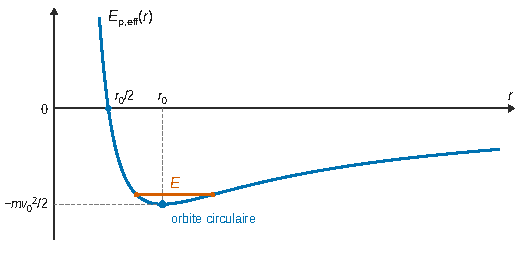
\includegraphics{figures/q09-potentiel-effectif.pdf}
\caption*{Figure 1 --- Énergie potentielle effective : minimum en \(r_0\) (orbite
circulaire), petites oscillations de \(r\) autour}
\end{figure}

\hypertarget{question-10}{%
\subsection{Question 10}\label{question-10}}

On dérive par rapport au temps l'énergie \(E=\frac12m\dot r^2+E_{p,\text{eff}}(r)\), constante. Pour \(\dot r\neq0\) :

\equationajustee{m\ddot r=-E_{p,\text{eff}}'(r) .}

On pose \(r=r_0+r_1\). Le développement limité au premier ordre en \(r_1\) donne \(E_{p,\text{eff}}'(r_0+r_1)\simeq E_{p,\text{eff}}''(r_0)\,r_1\), puisque \(E_{p,\text{eff}}'(r_0)=0\). Or

\equationajustee{\begin{aligned}
E_{p,\text{eff}}''(r_0)&=\frac{3mv_0^2r_0^2}{r_0^4}-\frac{2mv_0^2r_0}{r_0^3}\\
&=\frac{mv_0^2}{r_0^2}
\end{aligned}}

D'où l'équation d'un oscillateur harmonique :

\equationajustee{\ddot r_1+\frac{v_0^2}{r_0^2}\,r_1=0}

\equationajustee{\boxed{\omega=\frac{v_0}{r_0}}}

C'est la pulsation orbitale : la période radiale égale la période de révolution (orbite fermée).

\hypertarget{question-11}{%
\subsection{Question 11}\label{question-11}}

L'aphélie de DART doit valoir \(1{,}01\,r_0\), soit une amplitude \(|r_1|_{\max}=0{,}01\,r_0\). Comme \(|r_1|/r_0\le10^{-2}\ll1\), \textbf{l'approximation des petites oscillations est justifiée.}

\hypertarget{question-12}{%
\subsection{Question 12}\label{question-12}}

La solution générale s'écrit \(r_1(t)=A\cos(\omega t+\phi)\). L'impulsion est donnée à \(t=0\) sur l'orbite circulaire : \(r_1(0)=0\) et \(\dot r_1(0)=v_1\). D'où

\equationajustee{r_1(t)=\frac{v_1}{\omega}\sin(\omega t) .}

L'amplitude vaut \(|v_1|/\omega=r_0|v_1|/v_0\). On impose qu'elle égale \(0{,}01\,r_0\) :

\equationajustee{\boxed{|v_1|=0{,}01\,v_0=300\ \text{m·s}^{-1}}}

\hypertarget{question-13}{%
\subsection{Question 13}\label{question-13}}

\equationajustee{\begin{aligned}
T_{\text{DART}}&=\frac{2\pi}{\omega}=\frac{2\pi r_0}{v_0}\\
&=\frac{2\pi\times1{,}5\times10^{11}}{3\times10^4}\ \text{s}\\
&\approx3{,}1\times10^7\ \text{s}
\end{aligned}}

\equationajustee{\boxed{T_{\text{DART}}\approx1\ \text{an}}}

Sans calcul : le demi-grand axe est inchangé au premier ordre (Q7). D'après la troisième loi de Kepler, la période est celle de la Terre, un an.

\hypertarget{question-14}{%
\subsection{Question 14}\label{question-14}}

Entre l'impulsion et l'impact s'écoulent 3/4 d'année, soit \(\frac34T_{\text{DART}}\). L'impact a lieu à l'aphélie de DART, maximum de \(r_1(t)=A\sin(\omega t)\) avec \(A=v_1/\omega\), du signe de \(v_1\).

\begin{itemize}
\tightlist
\item
  Si \(v_1>0\) (vers l'extérieur), \(A>0\) : le maximum est atteint à \(\omega t=\pi/2\), soit \(t=T/4\).
\item
  Si \(v_1<0\) (vers le Soleil), \(A<0\) : \(r_1\) devient d'abord négatif (périhélie à \(T/4\)), et le maximum est atteint à \(\omega t=3\pi/2\), soit \(t=3T/4\).
\end{itemize}

\begin{figure}[H]
\centering
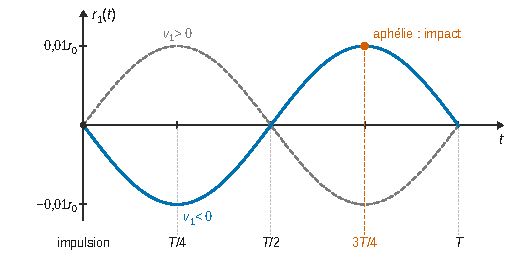
\includegraphics{figures/q14-oscillation-radiale.pdf}
\caption*{Figure 2 --- Écart radial \(r_1(t)\) : l'aphélie est atteint à \(T/4\)
si \(v_1>0\), à \(3T/4\) si \(v_1<0\)}
\end{figure}

L'aphélie est atteint \(3T/4\) après l'impulsion, donc \(A<0\) et \(v_1<0\) : \textbf{l'impulsion était dirigée vers le Soleil.}

\hypertarget{seconde-muxe9thode-constantes-du-mouvement}{%
\subsection{Seconde méthode : constantes du mouvement}\label{seconde-muxe9thode-constantes-du-mouvement}}

\hypertarget{question-15}{%
\subsection{Question 15}\label{question-15}}

On traite une trajectoire quelconque. Le principe fondamental de la dynamique et la dérivée du vecteur de base donnent

\equationajustee{m\frac{\mathrm d\vec v}{\mathrm dt}=-\frac{GM_\odot m}{r^2}\vec e_r}

\equationajustee{\frac{\mathrm d\vec e_\theta}{\mathrm dt}=-\dot\theta\,\vec e_r}

Pour \(B\) constant, en utilisant \(\dot\theta=L/(mr^2)\) (conservation du moment cinétique) :

\equationajustee{\begin{aligned}
\frac{\mathrm d\vec T}{\mathrm dt}&=\left(-\frac{GM_\odot}{r^2}+B\dot\theta\right)\vec e_r\\
&=\frac{1}{r^2}\left(-GM_\odot+\frac{BL}{m}\right)\vec e_r
\end{aligned}}

Ce vecteur est nul à tout instant si et seulement si

\equationajustee{\boxed{B=\frac{GM_\odot m}{L}}}

\(B\) ne dépend que de la trajectoire (par \(L\)), et pour cette valeur \(\vec T\) est constant.

\hypertarget{question-16}{%
\subsection{Question 16}\label{question-16}}

Sur l'orbite circulaire de rayon \(r_0\), \(L=mr_0v_0\) et \(GM_\odot=v_0^2r_0\), donc \(B=v_0\). Comme \(\vec v=v_0\vec e_\theta\) :

\equationajustee{\boxed{B=v_0}}

\equationajustee{\boxed{\vec T=\vec 0}}

\hypertarget{question-17}{%
\subsection{Question 17}\label{question-17}}

\begin{figure}[H]
\centering
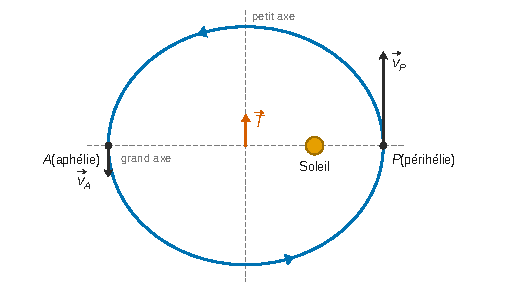
\includegraphics{figures/q17-orbite-vecteur-t.pdf}
\caption*{Figure 3 --- Orbite elliptique : Soleil au foyer, sens de parcours,
\(\vec v_P\), \(\vec v_A\) et \(\vec T\) porté par le petit axe}
\end{figure}

Le Soleil occupe le \textbf{foyer} proche du périhélie \(P\) ; l'aphélie \(A\) est le sommet opposé ; l'orbite est parcourue dans le sens trigonométrique.

Direction. \(\vec T\) est constant : on l'évalue aux deux apsides, où la vitesse est orthoradiale, \(\vec v=v\,\vec e_\theta\). En \(A\), \(\vec e_\theta(A)=-\vec e_\theta(P)\). D'où

\equationajustee{\begin{aligned}
\vec T&=(v_P-B)\,\vec e_\theta(P)&&\text{(au \text{périhélie})}\\
\vec T&=(B-v_A)\,\vec e_\theta(P)&&\text{(\text{à} l'\text{aphélie})}
\end{aligned}}

\(\vec T\) est colinéaire à \(\vec e_\theta(P)\), orthogonal au grand axe :

\equationajustee{\boxed{\vec T\ \text{est \text{dirigé} selon le petit axe}}}

Sens. L'égalité des deux expressions donne \(B=\frac12(v_P+v_A)\), puis \(\vec T=\frac12(v_P-v_A)\,\vec e_\theta(P)\). La conservation du moment cinétique aux apsides s'écrit \(mr_Pv_P=mr_Av_A\). Comme \(r_P<r_A\), on a \(v_P>v_A\) : \textbf{\(\vec T\) a le sens de la vitesse au périhélie.}

\hypertarget{question-18}{%
\subsection{Question 18}\label{question-18}}

Le moment cinétique \(L=mr_0v_0\) est inchangé (Q6), donc \(B=GM_\odot m/L=v_0\). À l'instant de l'impulsion, \(\vec v=v_1\vec e_r+v_0\vec e_\theta\), donc \(\vec T=v_1\vec e_r\) :

\equationajustee{\boxed{B=v_0}}

\equationajustee{\boxed{|\vec T|=|v_1|}}

\hypertarget{question-19}{%
\subsection{Question 19}\label{question-19}}

D'après Q17, aux apsides \(\vec v\) est colinéaire à \(\vec T\) : de même sens au périhélie, de sens opposé à l'aphélie. Donc \(v_P=B+|\vec T|\) et \(v_A=B-|\vec T|\) :

\equationajustee{\boxed{v_P=v_0+|v_1|}}

\equationajustee{\boxed{v_A=v_0-|v_1|}}

\hypertarget{question-20}{%
\subsection{Question 20}\label{question-20}}

Le \textbf{moment cinétique} (loi des aires). Aux apsides, \(\vec v\perp\vec r\), donc \(L=mrv\). Sa valeur est celle de l'orbite initiale, \(L=mr_0v_0\), inchangée par l'impulsion (Q6). À l'aphélie, \(mr_Av_A=mr_0v_0\), et \(v_A\) est donné par Q19 :

\equationajustee{\boxed{r_A=\frac{r_0v_0}{v_0-|v_1|}}}

De même, \(r_P=r_0v_0/(v_0+|v_1|)\).

\hypertarget{question-21}{%
\subsection{Question 21}\label{question-21}}

Développement limité au premier ordre en \(|v_1|/v_0\ll1\) :

\equationajustee{\begin{aligned}
r_A&=r_0\left(1-\frac{|v_1|}{v_0}\right)^{-1}\\
&\simeq r_0\left(1+\frac{|v_1|}{v_0}\right)
\end{aligned}}

Imposer \(r_A=1{,}01\,r_0\) donne \(|v_1|=0{,}01\,v_0\) : \textbf{on retrouve le résultat de la question 12.}

\hypertarget{iii-moteur-ionique}{%
\section{III --- Moteur ionique}\label{iii-moteur-ionique}}

\hypertarget{question-22}{%
\subsection{Question 22}\label{question-22}}

Théorème de la quantité de mouvement à force constante : \(M\,\Delta v=F\,\Delta t\), avec \(\Delta v=|v_1|=300\) m·s\(^{-1}\).

\equationajustee{\begin{aligned}
\Delta t&=\frac{M|v_1|}{F}=\frac{600\times300}{0{,}2}\ \text{s}\\
&=9\times10^5\ \text{s}
\end{aligned}}

\equationajustee{\boxed{\Delta t\approx10\ \text{jours}}}

Il faut comparer cette durée à l'échelle de temps du mouvement orbital : la période \(T\approx1\) an, ou plus finement \(1/\omega=r_0/v_0=5\times10^6\) s, soit environ 58 jours.

On a \(\Delta t/T\approx3\,\%\) et \(\Delta t/(1/\omega)\approx0{,}17\) : pendant la poussée, la direction du Soleil ne tourne que d'environ \(10°\). \textbf{L'impulsion peut être qualifiée de brève en première approximation.}

\hypertarget{question-23}{%
\subsection{Question 23}\label{question-23}}

Conservation de la charge :

\equationajustee{\frac{\partial\rho}{\partial t}+\operatorname{div}\vec j=0 .}

En régime stationnaire, \(\operatorname{div}\vec j=0\).

Les plaques sont grandes et les ions répartis uniformément sur leur surface : invariance par translation selon \(y\) et \(z\), d'où \(\vec j=j(x)\vec u_x\). Alors \(\dfrac{\mathrm dj}{\mathrm dx}=0\), et \(j\) est indépendante de \(x\).

Le courant est porté par les ions, de densité volumique de \textbf{charge} \(\rho(x)\) :

\equationajustee{\boxed{j=\rho(x)\,v(x)=\text{constante}}}

\hypertarget{question-24}{%
\subsection{Question 24}\label{question-24}}

Théorème de l'énergie cinétique pour un ion entre \(x=0\) (vitesse négligeable, \(V=0\)) et \(x\). La force électrique dérive de l'énergie potentielle \(eV\) :

\equationajustee{\tfrac12mv(x)^2-0=-\left(eV(x)-0\right)}

\equationajustee{\boxed{\tfrac12mv(x)^2=-eV(x)}}

Le signe est cohérent : \(V(x)\le0\) entre les plaques, et l'ion positif est accéléré vers les potentiels décroissants.

\hypertarget{question-25}{%
\subsection{Question 25}\label{question-25}}

Pendant \(\mathrm dt\), le nombre d'ions traversant \(S\) est \(\dfrac{jS}{e}\mathrm dt\), chacun portant la quantité de mouvement \(mv(x)\vec u_x\) :

\equationajustee{\boxed{F(x)=\frac{Sjm}{e}\,v(x)}}

Comme \(v(0)=0\) :

\equationajustee{\boxed{F(0)=0}}

Bilan pour les ions situés entre les plaques, en régime stationnaire : ils reçoivent par unité de temps la quantité de mouvement \(F(d)-F(0)=F(d)\) selon \(+\vec u_x\). Le moteur exerce donc sur eux la force \(F(d)\vec u_x\). Par la loi des actions réciproques, les ions exercent sur le moteur la force \(-F(d)\vec u_x\).

\textbf{La poussée vaut \(F(d)\) et est dirigée selon \(-\vec u_x\)}, à l'opposé de l'éjection des ions.

\begin{figure}[H]
\centering
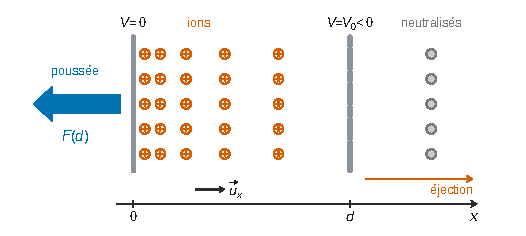
\includegraphics{figures/q25-moteur-ionique.pdf}
\caption*{Figure 4 --- Moteur ionique : ions accélérés de \(x=0\) à \(x=d\) puis
éjectés vers \(+x\), poussée \(F(d)\) selon \(-\vec u_x\)}
\end{figure}

\hypertarget{question-26}{%
\subsection{Question 26}\label{question-26}}

On dérive \(\frac12mv^2=-eV\) par rapport à \(x\), avec \(E=-\mathrm dV/\mathrm dx\) :

\equationajustee{mvv'=-eV'=eE}

\equationajustee{\boxed{v'(x)=\frac{eE(x)}{mv(x)}}}

\hypertarget{question-27}{%
\subsection{Question 27}\label{question-27}}

Maxwell-Gauss à une dimension, puis Q23 : \(E'=\rho/\varepsilon_0=j/(\varepsilon_0v)\). Donc

\equationajustee{\begin{aligned}
\frac{\mathrm d}{\mathrm dx}\left(\tfrac12\varepsilon_0E^2\right)&=\varepsilon_0EE'=\frac{jE}{v}\\
\frac{\mathrm d}{\mathrm dx}\left(\frac{F}{S}\right)&=\frac{jm}{e}\,v'=\frac{jm}{e}\cdot\frac{eE}{mv}=\frac{jE}{v}
\end{aligned}}

D'où \(\dfrac{\mathrm dQ}{\mathrm dx}=0\) : \textbf{\(Q\) est indépendant de \(x\).} On l'évalue en \(x=0\), où \(F(0)=0\) :

\equationajustee{\boxed{Q=\tfrac12\varepsilon_0E(0)^2\ge0}}

\hypertarget{question-28}{%
\subsection{Question 28}\label{question-28}}

Comme \(E'=\rho/\varepsilon_0>0\), \(E\) croît avec \(x\), et \(E(0)\ge0\) (les ions partent du repos vers \(+x\)).

La contrainte \(|E|\le E_{\max}\) porte donc sur \(E(d)\). En \(x=d\), puisque \(Q\ge0\) :

\equationajustee{\frac{F(d)}{S}=\tfrac12\varepsilon_0E(d)^2-Q\le\tfrac12\varepsilon_0E_{\max}^2}

L'égalité exige \(Q=0\) et \(E(d)=E_{\max}\) : la poussée maximale est atteinte pour \(Q=0\) et vaut

\equationajustee{\boxed{F_{\max}=\tfrac12\varepsilon_0E_{\max}^2S}}

\hypertarget{question-29}{%
\subsection{Question 29}\label{question-29}}

Avec \(Q=0\), la relation de Q27 devient \(\frac12\varepsilon_0E^2=F/S=\dfrac{jm}{e}v\). On y porte \(E=-V'\) et \(v=\sqrt{-2eV/m}\) (Q24), avec \(\dfrac me\sqrt{\dfrac{2e}{m}}=\sqrt{\dfrac{2m}{e}}\) :

\equationajustee{\boxed{\tfrac12\varepsilon_0\left(\frac{\mathrm dV}{\mathrm dx}\right)^2=j\sqrt{\frac{2m}{e}}\,\sqrt{-V(x)}}}

\hypertarget{question-30}{%
\subsection{Question 30}\label{question-30}}

On essaie \(V=V_0(x/d)^\beta\) avec \(V_0<0\) :

\equationajustee{\begin{aligned}
V'&=\frac{\beta V_0}{d}\left(\frac xd\right)^{\beta-1}\\
\sqrt{-V}&=\sqrt{-V_0}\left(\frac xd\right)^{\beta/2}
\end{aligned}}

L'équation s'écrit

\equationajustee{\frac{\varepsilon_0\beta^2V_0^2}{2d^2}\left(\frac xd\right)^{2\beta-2}=j\sqrt{\frac{2m}{e}}\sqrt{-V_0}\left(\frac xd\right)^{\beta/2}}

Elle est vérifiée pour tout \(x\) si \(2\beta-2=\beta/2\), soit

\equationajustee{\boxed{\beta=\frac43}}

et si les coefficients sont égaux, ce qui fixe la densité de courant (loi de Child-Langmuir) :

\equationajustee{j=\frac{4\varepsilon_0}{9d^2}\sqrt{\frac{2e}{m}}\,(-V_0)^{3/2}}

Cette forme vérifie \(V(0)=0\), \(V(d)=V_0\) et \(V'(0)=0\), c'est-à-dire \(E(0)=0\), cohérent avec \(Q=\frac12\varepsilon_0E(0)^2=0\).

\hypertarget{question-31}{%
\subsection{Question 31}\label{question-31}}

Sans charge d'espace, \(V''=0\) : \(V=V_0\,x/d\) (droite, champ uniforme). Avec charge d'espace, \(V=V_0(x/d)^{4/3}\). Dans les deux cas, \(V\) est \textbf{négatif} entre les plaques.

\begin{longtable}[]{@{}llllll@{}}
\toprule\noalign{}
\(x/d\) & 0 & 0,25 & 0,5 & 0,75 & 1 \\
\midrule\noalign{}
\endhead
\bottomrule\noalign{}
\endlastfoot
\(V/V_0\) (charge d'espace) & 0 & 0,16 & 0,40 & 0,68 & 1 \\
\(V/V_0\) (vide) & 0 & 0,25 & 0,50 & 0,75 & 1 \\
\end{longtable}

\begin{figure}[H]
\centering
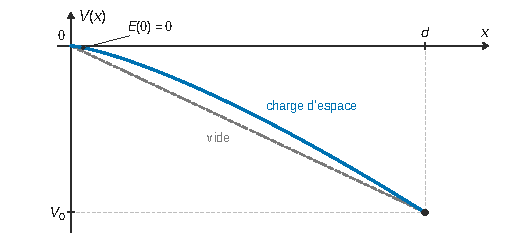
\includegraphics{figures/q31-potentiel-child-langmuir.pdf}
\caption*{Figure 5 --- Potentiel \(V(x)\) : charge d'espace (\(V_0(x/d)^{4/3}\),
tangente horizontale en 0) et condensateur vide (droite)}
\end{figure}

Comme \(V_0<0\) et \((x/d)^{4/3}<x/d\) sur \(]0,d[\), la courbe avec charge d'espace reste \textbf{au-dessus} de la droite.

Elle part avec une \textbf{tangente horizontale} (\(E(0)=0\)) et arrive en \(x=d\) plus raide que la droite : pente \(\frac43V_0/d\), soit \(E(d)=\frac43|V_0|/d\).

\hypertarget{iv-uxe9tude-de-lastuxe9rouxefde-double-didymos-dimorphos-et-effet-de-limpact-de-dart}{%
\section{IV --- Étude de l'astéroïde double Didymos-Dimorphos et effet de l'impact de DART}\label{iv-uxe9tude-de-lastuxe9rouxefde-double-didymos-dimorphos-et-effet-de-limpact-de-dart}}

\hypertarget{question-32}{%
\subsection{Question 32}\label{question-32}}

La luminosité est proportionnelle à la surface éclairée vue depuis la Terre, donc aux sections \(\pi R^2\). Hors creux, elle est proportionnelle à \(R_1^2+R_2^2\). Lors du second creux, S est caché derrière Didymos : elle est proportionnelle à \(R_1^2\). La baisse relative vaut donc

\equationajustee{\frac{R_2^2}{R_1^2+R_2^2}=0{,}04}

\equationajustee{\frac{R_2^2}{R_1^2}=\frac{0{,}04}{0{,}96}=\frac{1}{24}}

\equationajustee{\boxed{\frac{R_2}{R_1}\approx0{,}2}}

\hypertarget{question-33}{%
\subsection{Question 33}\label{question-33}}

On repère S par l'angle \(\varphi=2\pi t/P\) compté depuis la conjonction (S derrière Didymos). Vue de la Terre, très lointaine, la distance projetée entre les centres vaut \(D|\sin\varphi|\).

\begin{itemize}
\tightlist
\item
  S est entièrement caché tant que \(D|\sin\varphi|<R_1-R_2\).
\item
  S est partiellement caché tant que \(D|\sin\varphi|<R_1+R_2\).
\end{itemize}

Sur la figure 2, le second creux dure environ \(0{,}15\,P\) entre premier et dernier contact, et environ \(0{,}09\,P\) en fond plat. D'où

\equationajustee{\frac{R_1+R_2}{D}\approx\sin(0{,}15\,\pi)\approx0{,}45}

\equationajustee{\frac{R_1-R_2}{D}\approx\sin(0{,}09\,\pi)\approx0{,}28}

\equationajustee{\boxed{\frac{R_1}{D}\approx0{,}35\ \text{\text{à}}\ 0{,}4}}

On obtient aussi \(R_2/D\approx0{,}08\), soit \(R_2/R_1\approx0{,}2\), cohérent avec Q32.

Dessin à l'échelle (figure 6, avec \(R_1\approx0{,}37\,D\) et \(R_2\approx0{,}08\,D\)) : le système est compact, Didymos occupe plus du tiers du rayon orbital.

\begin{figure}[H]
\centering
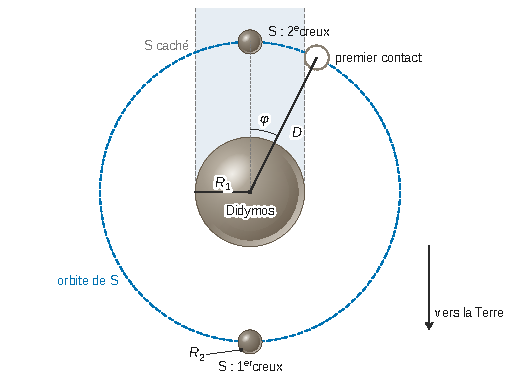
\includegraphics{figures/q33-asteroide-double-echelle.pdf}
\caption*{Figure 6 --- Astéroïde double à l'échelle (\(R_1\approx0{,}37\,D\),
\(R_2\approx0{,}08\,D\)) et zone où S est caché vu de la Terre}
\end{figure}

\hypertarget{question-34}{%
\subsection{Question 34}\label{question-34}}

Les deux creux correspondent à S devant puis derrière Didymos. Sur une orbite circulaire, ils sont séparés d'une demi-révolution : \(\Delta t=P/2\) (la figure le confirme, creux centrés vers \(0{,}25\) et \(0{,}75\)). On en tire \(P=2\Delta t\).

La masse de S est négligeable devant \(M_1=\frac43\pi R_1^3\rho_1\), puisque \((R_2/R_1)^3\approx10^{-2}\). Pour S en orbite circulaire autour de Didymos, le principe fondamental de la dynamique donne

\equationajustee{\begin{aligned}
\left(\frac{2\pi}{P}\right)^2D&=\frac{GM_1}{D^2}\\
&=\frac{4\pi G\rho_1}{3}\,\frac{R_1^3}{D^2}
\end{aligned}}

\equationajustee{\boxed{\rho_1=\frac{3\pi}{GP^2}\left(\frac{D}{R_1}\right)^3=\frac{3\pi}{4G\,\Delta t^2}\left(\frac{D}{R_1}\right)^3}}

\(R_1/D\) venant de Q33, \textbf{\(\rho_1\) est déterminée par la seule mesure de \(\Delta t\).} Avec une période d'environ 12 h et \(R_1/D\approx0{,}33\), on trouve \(\rho_1\sim2\times10^3\) kg·m\(^{-3}\).

\hypertarget{question-35}{%
\subsection{Question 35}\label{question-35}}

On différencie la troisième loi de Kepler, \(T^2\propto a^3\) : \(\dfrac{\Delta T}{T}=\dfrac32\dfrac{\Delta a}{a}\). D'où

\equationajustee{\boxed{\frac{\Delta a}{a}=\frac23\times4{,}8\,\%=+3{,}2\,\%}}

Juste après l'impact, S est toujours à la distance \(D\). L'énergie mécanique s'écrit

\equationajustee{\tfrac12v^2-\frac{GM_1}{D}=-\frac{GM_1}{2a}}

\equationajustee{v^2=GM_1\left(\frac2D-\frac1a\right)}

Avant l'impact, l'orbite est circulaire : \(a=D\) et \(v^2=GM_1/D\). En différentiant à \(D\) fixé :

\equationajustee{\begin{aligned}
2v\,\Delta v&=\frac{GM_1}{a^2}\,\Delta a\\
\frac{\Delta v}{v}&=\frac{GM_1}{2v^2a^2}\,\Delta a=\frac12\,\frac{\Delta a}{a}
\end{aligned}}

\equationajustee{\boxed{\frac{\Delta v}{v}=+1{,}6\,\%}}

La vitesse de S a augmenté en norme, sans changer de direction. DART, de vitesse parallèle à celle de S, \textbf{a percuté S dans le sens de son mouvement} (en le rattrapant par l'arrière). Si la période avait diminué (cas de la mission réelle), on aurait conclu à un impact de face, en sens opposé au mouvement de S.

\end{document}
